%  ----------------------------------------------------------------------------
% Dieses Dokument ist eine Kurzversion von:
%
% Copyright (c) 2016 by Burkhardt Renz. All rights reserved.
% Vorlage Abschlussarbeit THM (minimal)
% $Id: vorlage.tex 3811 2016-08-05 12:03:51Z br $
% 
% Der Dokumentstyle wurde von "srcbook" auf "article" geändert, 
% um den Einstieg in LaTex zu erleichtern. 
% Die Unterdateien wurden nicht per \input ins Dokument geholt, 
% sondern direkt eingefügt. Chapters wurden in Sections 
% umbenannt. Das Titelblatt wurde verändert.
% Die Beschreibung der labeling-Umgebung wurde entfernt. ----------------------------------------------------------------------------

\documentclass[11pt]{scrartcl}       % KOMA-Skript für Artikel
\RequirePackage{filecontents}

%% Präambel
\usepackage[english, ngerman]{babel} % deutsche typogr. Regeln + Trenntabelle
\usepackage[T1]{fontenc}             % interner TeX-Font-Codierung
\usepackage{lmodern}                 % Font Latin Modern
\usepackage[utf8]{inputenc}          % Font-Codierung der Eingabedatei
\usepackage[babel]{csquotes}         % Anführungszeichen
\usepackage{graphicx}                % Graphiken
\usepackage{booktabs}                % Tabellen schöner
\usepackage{listingsutf8}            % Listings mit Einstellungen
\usepackage[
backend=biber,			% Biber Compiler
style=alphabetic,  		% alphanumeric Labels
sorting=anyt 			% sort by alphabetic label, name, year, title 
]{biblatex}				% BibLaTex
\addbibresource{References.bib}

\lstset{basicstyle=\small\ttfamily,
	tabsize=2,
	basewidth={0.5em,0.45em},
	extendedchars=true}
\usepackage{amsmath}	               % Mathematik
\usepackage[pdftex]{hyperref}       
\hypersetup{
	bookmarksopen=true,
	bookmarksopenlevel=3,
	colorlinks,
	citecolor=blue,
	linkcolor=blue,
}
\usepackage{scrhack}								 % unterdrückt Fehlermeldung von listings

%% Nummerierungstiefen
\setcounter{tocdepth}{3}             % 3 Stufen im Inhaltsverzeichnis
\setcounter{secnumdepth}{3} 		 % 3 Stufen in Abschnittnummerierung

% ----------------------------------------------------------------------------
\begin{document}



%% Titelseite
	
\titlehead{

\includegraphics[width=0.9\textwidth]{img/mni-logo}
}
\title{Einige wesentliche Kriterien für die Auswahl von Software für ein QMS}
\author{Assem Hussein}
\date{Winter 2021/2022}
\maketitle	


\newpage
%% Verzeichnissse
 \tableofcontents
%% \listoffigures
%% \listoftables
%\lstlistoflistings

\newpage

\section{Einleitung}
Die Auswahl eines wirksamen QMS ist eine nicht triviale Herausforderung, die einen besonderen Ansatz erfordert. Immer mehr Organisationen streben täglich danach, ein QMS einzuführen und sich zertifizieren zu lassen. Heute übersteigt die Zahl der zertifizierten QMS 1,5 Millionen \cite{Leontyuk_2019}. Ein solch gravierender Trend muss sich bei der Erfüllung der gesetzlichen Anforderungen als wirksam erwiesen haben und gleichzeitig die Kundenzufriedenheit erhöhen, was wiederum zu höheren Gewinnen führt.
\\
\\
Hierbei werden allgemeine Verfahren für die Softwareauswahl vorgestellt und die Hauptkriterien der Softwareauswahl erläutert. Insbesondere werden die wesentlichen Kriterien für die Auswahl eines QMS im Detail betrachtet.


\section{Allgemeines Verfahren für die Softwareauswahl}

TODO


\subsection{Gängige Ansätze}

TODO


\subsection{Allgemeine Kriterien}

TODO

 

\subsubsection{Kriterium/Kategorie A}

TODO


\subsubsection{Kriterium/Kategorie B}

TODO


\subsubsection{Kriterium/Kategorie C}

TODO


\subsubsection{Kriterium/Kategorie D}

TODO

\newpage
\section{Was ist ein QMS?}
\subsection{Definition und Anwendungsgebiet}
Ein Qualitätsmanagementsystem (kurz: QMS) ist eine Methode der Unternehmensführung. Ziel ist ein systematisches Qualitätsmanagement. Bei der Einführung muss das QMS gezielt auf das Produkt oder die erbrachte Dienstleistung zugeschnitten sein, d. h. es ist wichtig, dass es den Anforderungen des Betriebs gerecht wird. Um jedoch eine korrekte Umsetzung zu gewährleisten, gibt es einige allgemeine Richtlinien in Form der ISO 9001:2015 \cite{normungsinstitut2009qualitatsmanagementsysteme}, die helfen sollen, die Implementierung eines QMS zu standardisieren. Das am weitesten verbreitete Modell ist ein QMS, dessen Anforderungen
und Empfehlungen in der internationalen Norm ISO 9000 beschrieben sind \cite{sytko2017instrumentation}. 
\\
\\
Gemäß ISO 9000:2015 \cite{din20059000} wird das QMS wie folgt definiert:\
\begin{quotation}
„Ein QM-System umfasst Tätigkeiten, mit denen die Organisation ihre Ziele ermittelt und die Prozesse und Ressourcen bestimmt, die zum Erreichen der gewünschten Ergebnisse erforderlich sind. Das QMS führt und steuert in Wechselwirkung stehende Prozesse und Ressourcen, die erforderlich sind, um Wert zu schaffen und die Ergebnisse für relevante interessierte Parteien zu verwirklichen.“
\end{quotation}

%Auf ähnliche Weise erläutert \citeauthor{mai2020grundlage} in \citeyear{mai2020grundlage}, was ein QMS ist:
%
%\begin{quotation}
%„Ein Qualitätsmanagementsystem sollte alle Tätigkeiten umfassen, die dem Unternehmen ermöglichen, Ziele zu ermitteln und Prozesse sowie Ressourcen zu bestimmen, die zum Erreichen der Ziele notwendig sind. Das Qualitätsmanagementsystem ist eine strategische Entscheidung, Prozesse und Ressourcen wirksam und effizient zu lenken, um hieraus kurz-, mittel- und langfristige Erfolge zu verwirklichen und umzusetzen.“ \cite{mai2020grundlage}
%\end{quotation}

In diesem Sinne hilft ein QMS, die Aktivitäten einer Organisation zu koordinieren und zu steuern, um die Anforderungen von Kunden und Behörden zu erfüllen sowie ihre Wirksamkeit und Rentabilität kontinuierlich zu verbessern. Dies führt zu einer dauerhaften Verbesserung der Unternehmensleistung.

\subsection{Die Grundsätze des QMS}

Die Grundsätze des QMS sind in der DIN EN ISO 9000 beschrieben. Diese Grundsätze müssen bei der Einführung und Anwendung eines QMS im Unternehmen berücksichtigt werden, damit die Anforderungen der DIN EN ISO 9001 erfüllt werden können. Die sieben Grundsätze des Qualitätsmanagements \cite{mai2020grundlage} sind:

\begin{enumerate}

\item Kundenorientierung (Customer focus) \\
Der Kunde bestimmt die Anforderungen an die Produkte und Leistungen des
Unternehmens. D. h. Der nachhaltige Erfolg ist von der Zufriedenheit und
dem Vertrauen des Kunden abhängt.

\item Führung (Leadership) \\
Wenn ein bestimmtes Thema im Unternehmen umgesetzt werden soll, müssen die Führungskräfte Vorreiter in diesem Thema sein und die
Voraussetzungen dafür schaffen, dass die Kundenanforderungen umgesetzt werden können.

\item Einbeziehung von Personen (Engagement) \\
Eine ausführliche Information über den Grund von neuen Regelungen ist eine Mindestvoraussetzung. Wenn Mitarbeiter eine Regelung vorgesetzt bekommen und ihnen diese nicht sinnvoll erscheint, wird diese neue Regelung nicht gerne umgesetzt.

\item Prozessorientierter Ansatz (Process) \\
Jeder Prozess muss geplant, gesteuert, überwacht und verbessert werden.

\item Verbesserung (Improvement) \\
Ein wesentliches Ziel im Qualitätsmanagement ist einerseits die ständige Verbesserung der Produkte, andererseits der Organisation des Unternehmens. 

\item Faktengestützte Entscheidungsfindung (Evidence) \\
Aufgrund des Mangels an Daten werden viele Entscheidungen von Führungskräften intuitiv getroffen. Damit mehr dieser Entscheidungen auf einer soliden Grundlage stehen, sollen im Vorfeld grundlegende Daten ermittelt werden. 

\item Beziehungsmanagement (Relationship management) \\
Die interessierten Parteien beeinflussen die Unternehmensleistung. Je besser das Beziehungsmanagement ist, desto besser können die einzelnen Ansprüche gegeneinander abgewägt werden. Dies führt zu mehr Erfolg.
\end{enumerate}

\begin{figure}[!htb]
	\centering
	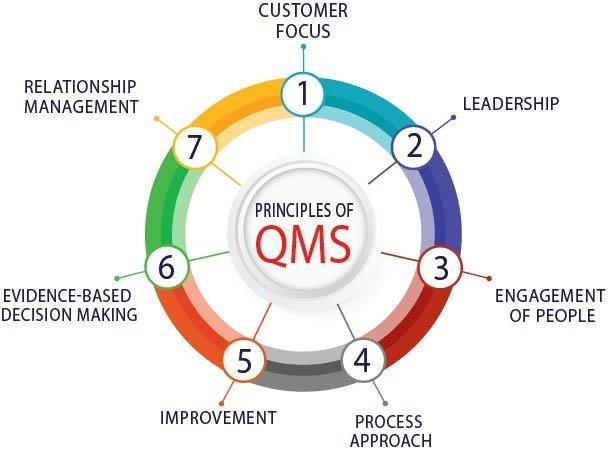
\includegraphics[width=.5\textwidth]{img/qms_iso9001.jpg}
	\caption{Die sieben Grundsätze des QMS}
\label{fig:qms_principles}
\end{figure}

%\begin{figure}
%\includegraphics[scale=0.6]{} 
%\caption{}
%\end{figure}



\subsection{Warum digitale QMS?}
Das traditionelle QMS ist die Grundlage für ein digitales QMS, jedoch durch Redundanz charakterisiert. Digitale QMS arbeitet in die Gegenrichtung, da es darauf ausgerichtet ist, Redundanz zu vermeiden \cite{ibrahim2019digital}. Digitale QMS unterstützen den abteilungsübergreifenden Datenfluss in einer Organisation auf automatisierte Weise und verringern die Notwendigkeit manueller Übertragungen, die anfällig für menschliche Fehler und zeitaufwändig sind. Digitale QMS ersetzen papiergestützte QMS, da sie auf Echtzeit-Messungen und Feedback-Mechanismen beruhen, die eine zeitnahe Reaktion auf Ausfälle und Fehler ermöglichen. \cite{yeung2003empirical}


\section{Wesentliche Kriterien für die Auswahl eines QMS}

TODO

\subsubsection{Kriterium A: Industriebranche}

TODO



\subsubsection{Kriterium B}

TODO



\subsubsection{Kriterium C}

 TODO



\subsubsection{Kriterium D}

 TODO



\section{Fazit}

 TODO



\newpage
\phantomsection
\addcontentsline{toc}{section}{Literatur}
%\nocite{*}
\printbibliography
\end{document}
% ----------------------------------------------------------------------------
